\section{Evietania Charis Sujadi}
\subsection{Fungsi Csv}
Fungsi csv yaitu memudahkan user dalam melakukan input data karena pada csv input data ataupun import data dalam skala besar dapat dilakukan dengan cara yang sederhana.
\subsection{Sejarah Csv}
Dari rilis pertama, Excel menggunakan format file biner yang disebut Binary Interchange File Format (BIFF) sebagai format file utamanya. Ini berubah ketika Microsoft merilis Office System 2007 yang memperkenalkan Office Open XML sebagai format file utamanya. Office Open XML adalah file kontainer berbasis XML yang mirip dengan XML Spreadsheets (XMLSS), yang diperkenalkan di Excel 2002. File versi XML tidak bisa menyimpan makro VBA. Meskipun mendukung format XML baru, Excel 2007 masih mendukung format lama yang masih berbasis BIFF tradisional. Selain itu Microsoft Excel juga mendukung format Comma Separated Values (CSV), DBase File (DBF), SYMbolic LinK (SYLK), Format Interchange Data (DIF) dan banyak format lainnya, termasuk format lembar kerja 1-2 Lotus - 3 (WKS, WK1, WK2, dll.) Dan Quattro Pro.
\lstinputlisting[firstline=7, lastline=20]{src/4/1174051/teori/gatau.py}
\subsection{Aplikasi yang dapat menghasilkan csv}
\begin{itemize}
\item Texteditor
Seperti notepad++,visual studio code,atom,sublime dan lain sebagainya
\item Program Spreadsheet
  Seperti excell,google spreadshare,LibreOfficecalc
 \end{itemize}
\subsection{Jelaskan bagaimana cara menulis dan membaca file csv di excel atau spreadsheet}
Caranya sangat mudah yaitu:
 Untuk menulisnya untuk yang paling atas itu kita buat headernya,untuk mepermudah membedakan datanya,dan untuk baris kedua dan seterusnya itu untuk data itu sendiri.Setelah di buat kalian save as kemudian pilih format CSV.Untuk membukan cukup di double clik file tersebut
\subsection{Jelaskan sejarah library csv}
CSV muncul untuk memudahkan data science dan analis karena dinilai terdapat banyak kemudahan yang didapat. CSV dapat dimaksimalkan jika dipaduka dengan python karena python adalah bahasa pemrograman yang support ke banyak library termasuk csv. Maka karena itulah perpaduan python dan csv seringkali digunakan oleh perusahaan-perushaan besar dalam mengolah datanya.
\subsection{Jelaskan sejarah library pandas}
Pandas merupakan tool yang dapat digunakan sebagai alat analisis data dan struktur untuk bahasa pemrograman Python. Pandas dapat mengolah data dengan mudah, salah satu fitur yang ada dalam pandas adalah Dataframe. Fitur dataframe dapat membaca sebuah file dan menjadikannya tabble, juga dapat mengolah suatu data dengan menggunakan operasi seperti join, group by dan teknik lainnya yang terdapat pada SQL. Dalam hal ini pandas tidak jauh beda dengan csv yaitu memiliki keunggulan dalam pengolahan data-data besar dan dapat disupport dengan baik dengan python walaupun mengimport data dalam jumlah banyak.
\subsection{Fungsi-fungsi Library CSV}
Dalam library csv terdapat dua fungsi yaiut fungsi membaca file dan menulis file csv.
Library csv mempunyai keunggulan dibandingkan format data lainnya adalah soal kompatibilitas. File csv dapat digunakan, diolah, diekspor/impor, dan dimodifikasi menggunakan berbagai macam perangkat lunak dan bahasa pemrograman. Pada library csv mempunyai fungsi import dan eksport data yang baik dan bisa digunakan dalam jumlah besar.
\subsection{Fungsi-fungsi library Pandas}
Pandas pun memiliki fungsi yang sama yaitu menulis dan membaca file. pandas menyediakan beragam fungsi operasi untuk mengolah data. Contoh jika menggunakan series bisa mencari nilai max, min, dan mean secara langsung, bahkan juga bisa melakukan operasi perpangkatan pada nilai Series secara langsung.
Pandas dapat mengolah suatu data dan mengolahnya seperti join, distinct, group by, agregasi, dan teknik seperti pada SQL. Hanya saja dilakukan pada tabel yang dimuat dari file ke RAM.
\subsection{Bukti Plagiarisme}
\begin{figure}[h]
	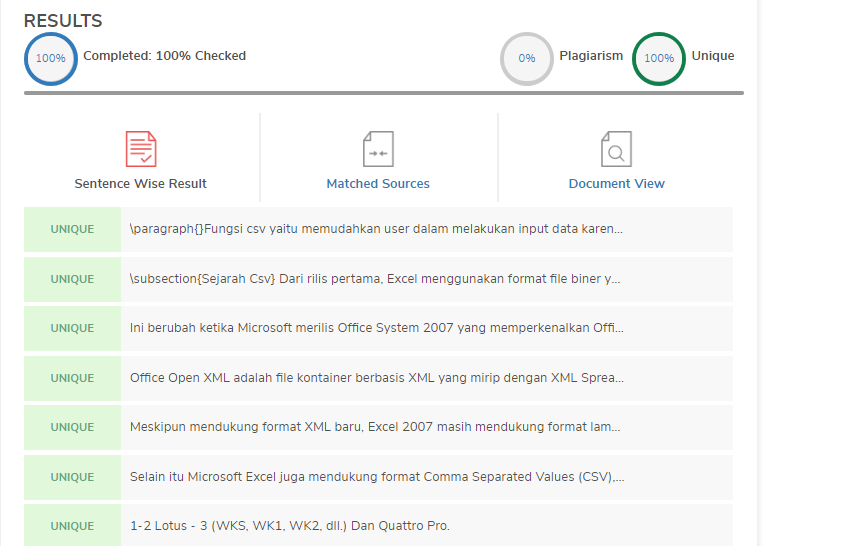
\includegraphics[width=10cm]{figures/4/1174051/teori/nih.png}
	\centering
\end{figure}
\section{Muhammad Dzihan Al-Banna}
\subsection{Soal 1}
Comma Separated Value atau CSV adalah format data yang memudahkan penggunanya melakukan input data ke database secara sederhana. CSV dapat digunakan dalam standar file ASCII. Dalam format csv record dipisahkan dengan tanda koma atau titik koma. Ketika user menerima file dengan format CSV, yang biasanya bertuliskan .CSV, maka file tersebut akan terbuka dalam format Microsoft Excel. CSV muncul demi memenuhi kebutuhan perusahaan-perusahaan besar dalam mengolah data yang banyak.
\lstinputlisting[firstline=7, lastline=20]{src/4/1174095/cobacsv.py}
\subsubsection{Fungsi}
Fungsi csv yaitu memudahkan user dalam melakukan input data karena di csv input data atau import data dalam skala besar dapat dilakukan dengan cara yang sederhana.
\subsection{Soal 2}
Ada beberapa aplikasi yang dapat menghasilkan file dengan format csv diantaranya google sheet, number di MacOS dan microsoft excel.
\subsection{Soal 3}
cara membuat file csv di excel cukup mudah yaitu :
\begin{itemize}
	\item Buat foldernya
	\item Pilih save as
	\item pilih file dengan format csv
\end{itemize}
cara membaca file di csv :
\begin{itemize}
	\item Klik data get external data form text
	\item Akan muncul Text Import Wizard, arahkan pada file csv yang ingin anda buka Open.
	\item Setelah File terbuka, akan muncul Text Import Wizard.
	\item Pilih Delimited, Kemudian Next (Di sini, bisa juga menentukan baris awal yang akan di import)
	\item Centrang pada Tab dan Comma (Atau sesuai pengaturan File Anda) Next.
	\item Atur Format data pada tiap kolom yang tampil dan klik Finish
\end{itemize}
\subsection{Soal 4}
CSV muncul untuk memudahkan data science dan analis karena dinilai terdapat banyak kemudahan yang didapat. CSV dapat dimaksimalkan jika dipaduka dengan python karena python adalah bahasa pemrograman yang support ke banyak library termasuk csv. Maka karena itulah perpaduan python dan csv seringkali digunakan oleh perusahaan-perushaan besar dalam mengolah datanya.
\subsection{Soal 5}
Pandas merupakan tool yang dapat digunakan sebagai alat analisis data dan struktur untuk bahasa pemrograman Python. Pandas dapat mengolah data dengan mudah, salah satu fitur yang ada dalam pandas adalah Dataframe. Fitur dataframe dapat membaca sebuah file dan menjadikannya tabble, juga dapat mengolah suatu data dengan menggunakan operasi seperti join, group by dan teknik lainnya yang terdapat pada SQL. Dalam hal ini pandas tidak jauh beda dengan csv yaitu memiliki keunggulan dalam pengolahan data-data besar dan dapat disupport dengan baik dengan python walaupun mengimport data dalam jumlah banyak.
\subsection{Soal 6}
Dalam library csv terdapat dua fungsi yaiut fungsi membaca file dan menulis file csv.
Library csv mempunyai keunggulan dibandingkan format data lainnya adalah soal kompatibilitas. File csv dapat digunakan, diolah, diekspor/impor, dan dimodifikasi menggunakan berbagai macam perangkat lunak dan bahasa pemrograman. Pada library csv mempunyai fungsi import dan eksport data yang baik dan bisa digunakan dalam jumlah besar.
\subsection{Soal 7}
Pandas pun memiliki fungsi yang sama yaitu menulis dan membaca file. pandas menyediakan beragam fungsi operasi untuk mengolah data. Contoh jika menggunakan series bisa mencari nilai max, min, dan mean secara langsung, bahkan juga bisa melakukan operasi perpangkatan pada nilai Series secara langsung.
Pandas dapat mengolah suatu data dan mengolahnya seperti join, distinct, group by, agregasi, dan teknik seperti pada SQL. Hanya saja dilakukan pada tabel yang dimuat dari file ke RAM.
\subsection{Bukti Plagiarisme}
\begin{figure}[h]
	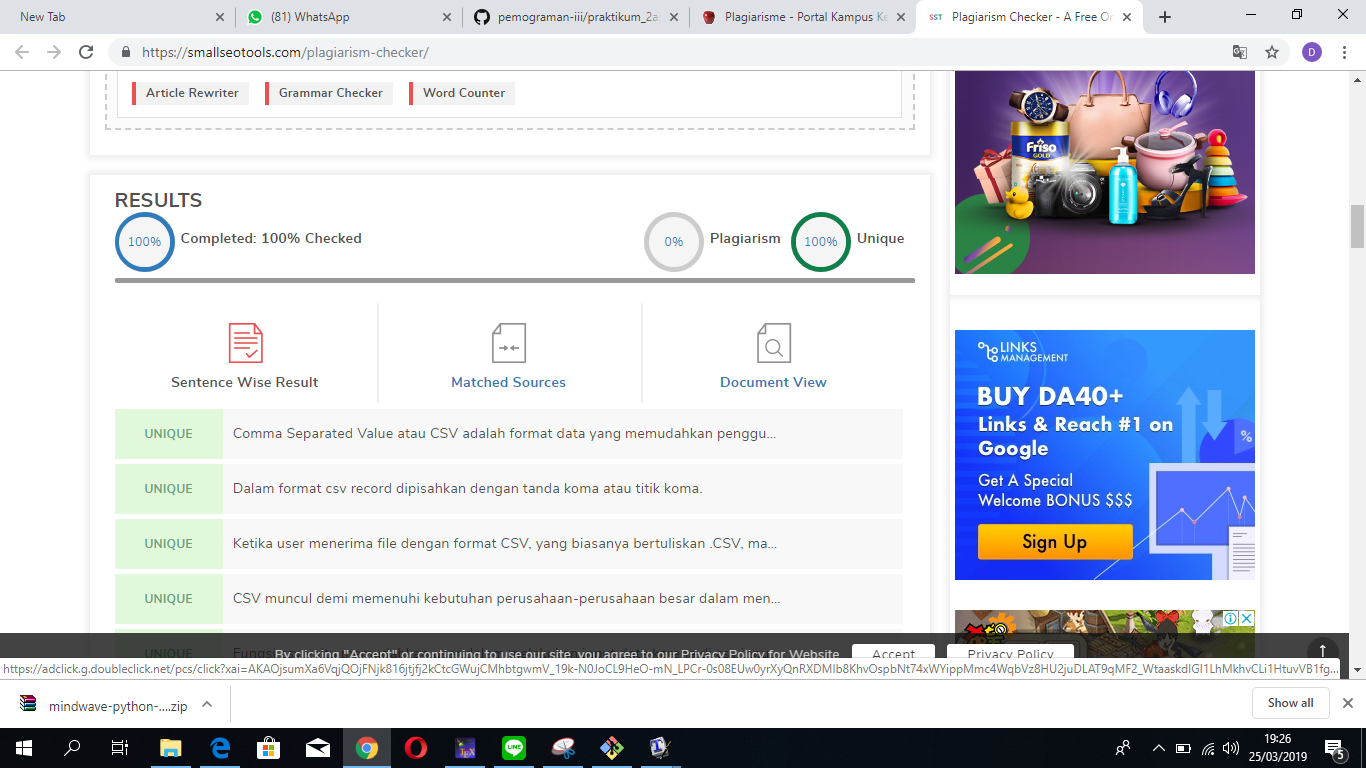
\includegraphics[width=10cm]{figures/4/1174095/bukti.png}
	\centering
\end{figure}

Kalau mau dibikin paragrap \textbf{cukup enter aja}, tidak usah pakai \verb|par| dsb

%\subsection{Soal 2}
%Isi jawaban soal ke-2

%\subsection{Soal 3}
%Isi jawaban soal ke-3

\section{Harun Ar-Rasyid}
\subsection{Soal 1}
Isi jawaban soal ke-1

Kalau mau dibikin paragrap \textbf{cukup enter aja}, tidak usah pakai \verb|par| dsb

%\subsection{Soal 2}
%Isi jawaban soal ke-2

%\subsection{Soal 3}
%Isi jawaban soal ke-3

\section{Sri Rahayu}
\subsection{Soal 1}
Isi jawaban soal ke-1

Kalau mau dibikin paragrap \textbf{cukup enter aja}, tidak usah pakai \verb|par| dsb

%\subsection{Soal 2}
%Isi jawaban soal ke-2

%\subsection{Soal 3}
%Isi jawaban soal ke-3

\section{Doli Jonviter}
\subsection{Soal 1}
Isi jawaban soal ke-1

Kalau mau dibikin paragrap \textbf{cukup enter aja}, tidak usah pakai \verb|par| dsb

%\subsection{Soal 2}
%Isi jawaban soal ke-2

%\subsection{Soal 3}
%Isi jawaban soal ke-3

\section{Rahmatul Ridha}
\subsection{Soal 1}
Isi jawaban soal ke-1

Kalau mau dibikin paragrap \textbf{cukup enter aja}, tidak usah pakai \verb|par| dsb

%\subsection{Soal 2}
%Isi jawaban soal ke-2

%\subsection{Soal 3}
%Isi jawaban soal ke-3

\section{Tomy Prawoto}
\subsection{Soal 1}
Isi jawaban soal ke-1

Kalau mau dibikin paragrap \textbf{cukup enter aja}, tidak usah pakai \verb|par| dsb

%\subsection{Soal 2}
%Isi jawaban soal ke-2

%\subsection{Soal 3}
%Isi jawaban soal ke-3
